% tous sur les makefiles
\subsection{Makefiles}

\begin{frame}{Motivations}
  \begin{itemize}
  \item Gérer plusieurs fichiers source et l'ensemble du processus de compilation / éditions des liens en une seule opération
  \begin{itemize}
  \item Faire plus ou moins l'équivalent des IDE comme Visual Studio
	\begin{itemize}
		\item Note : il y a moins bien (\texttt{make}), mais il y a aussi beaucoup mieux...
		\item VS ne sait pas gérer le multi-plateformes (et pour cause)
		\item VS ne sait pas trouver vos bibliothèques tout seul
	\end{itemize}
  \item Pour un gros projet : ne recompiler que le strict minimum nécessaire
  \end{itemize}
  \item Rappels : différentes phases
  \begin{itemize}
  \item Compilation des fichiers source (on a encouragé leur multiplication !)
  \item Edition des liens
  \end{itemize}

  \end{itemize}
\end{frame}

\begin{frame}{Principe}
  \begin{itemize}
  \item 2 étapes
  \begin{itemize}
  \item Ecriture d'un fichier \texttt{Makefile} (modifé à chaque fois qu'on ajoute un nouveau fichier source
  \item Compilation/Edition des liens : appel de la commande \texttt{make}
  \end{itemize}
  \begin{exampleblock}{Exemple}
  	Soit un programme exécutable \texttt{machin.out} construit à partir de 3 fichiers source \texttt{main.cxx}, \texttt{f1.cxx} et \texttt{f2.cxx}. Construction :
  	\begin{itemize}
  		\item \texttt{g++ -c main.cxx}
  		\item \texttt{g++ -c f1.cxx}
  		\item \texttt{g++ -c f2.cxx}
  		\item \texttt{g++ -o machin.out main.o f1.o f2.o}
  	\end{itemize}
  \end{exampleblock}
  \end{itemize}
\end{frame}

\begin{frame}{Graphe de dépendances}
  \begin{itemize}
  \item Ecrire quel fichier dépend de quel autre
  \begin{itemize}
  \item \texttt{machin.out} dépend de \texttt{main.o}, \texttt{f1.o} et \texttt{f2.o}
  \item \texttt{main.o} dépend de \texttt{main.cxx}
  \item \texttt{f1.o} dépend de \texttt{f1.cxx}
  \item \texttt{f2.o} dépend de \texttt{f2.cxx}
  \end{itemize}
  \item Les règles permettant de reconstruire les fichiers .out et .o sont connues
  \end{itemize}
      \begin{center}
      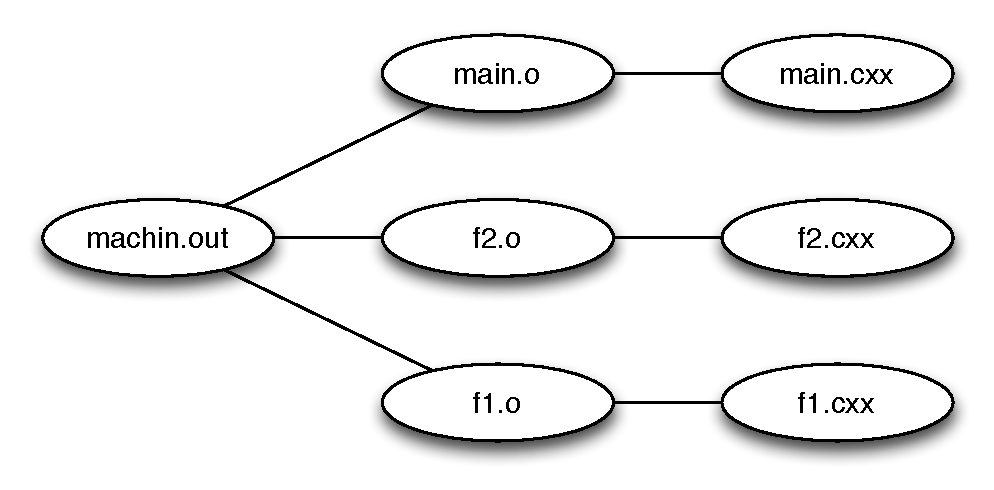
\includegraphics[scale=.43]{fig/base-dependance.pdf}
    \end{center}

\end{frame}

\begin{frame}{Dépendance temporelle}
  \begin{itemize}
  \item La date et l'heure du fichier sont utilisées : un fichier doit toujours être plus récent que les fichiers à sa droite dont il dépend
  \item Si ce n'est pas le cas, l'opération de production du fichier de gauche est lancée
  \item Le processus est itéré jusqu'à ce que toutes les règles soient respectées
  \end{itemize}
\end{frame}

\begin{frame}{Exemple (1/3)}
        \begin{center}
      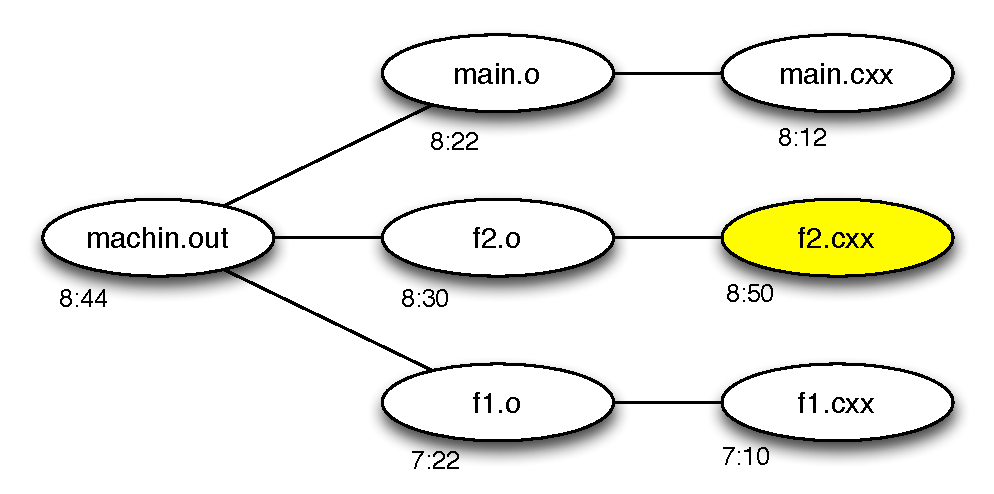
\includegraphics[scale=.6]{fig/base-dependance1.pdf}
    \end{center}
\end{frame}

\begin{frame}{Exemple (2/3)}
        \begin{center}
      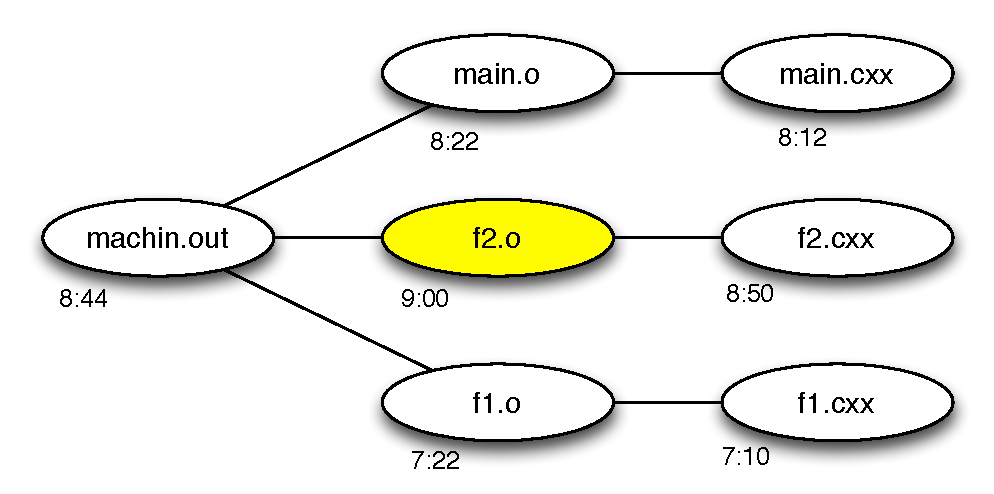
\includegraphics[scale=.6]{fig/base-dependance2.pdf}
    \end{center}
\end{frame}

\begin{frame}{Exemple (3/3)}
        \begin{center}
      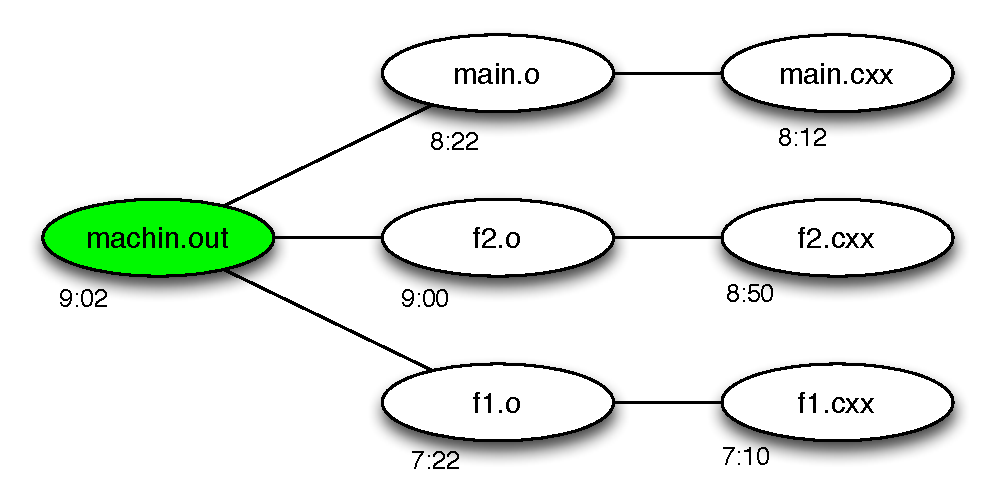
\includegraphics[scale=.6]{fig/base-dependance3.pdf}
    \end{center}
\end{frame}

\begin{frame}{Syntaxe du \texttt{Makefile}}
\begin{block}{Ensemble de règles de la forme}
\texttt{  fichier: fichier1 fichier2 fichier3 ... \\
  	<TAB>régle de production de fichier \\
}\end{block}
\begin{itemize}
\item Note : le fichier s'appelle obligatoirement \texttt{Makefile}
\begin{itemize}
\item Sauf parfois sous Windows, qui n'aime pas les fichiers sans extensions...
\end{itemize}
\item La première règle est toujours celle qui produit l'exécutable
\begin{itemize}
	\item en fait non, c'est juste celle qui sera vérifiée en premier par \texttt{make}
\end{itemize}
\item Ensuite il suffit d'appeler la commande \texttt{make}
\end{itemize}
\end{frame}

\begin{frame}[fragile]
  \frametitle{Makefile de l'exemple}
        \begin{center}
      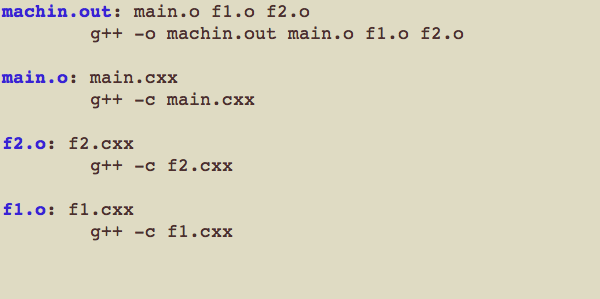
\includegraphics[scale=.4]{fig/makefile.png}
    \end{center}
\end{frame}
